\section[Wykład 13: 8-VI-2017 - Temat: Ekspandery]{Temat: Ekspandery}
\begin{definition}[Ekspander]
Ekspander to graf w którym najmniejsza niezerowa wartość własna Laplasjanu leży daleko od zera.\\
EKSPANDER $\rightarrow$ graf o równomiernie rozłożonych krawędziach
\end{definition}
\begin{figure}[H]
\centering
\begin{tikzpicture}
\coordinate (A) at (0.45,0);
\coordinate (B) at (1.5,0);
\coordinate (D) at (3.5,0);
\coordinate (E) at (6.5,0);

\draw[->] (0,0) -- (7,0);

\draw[thick] ($(A)+(0,5pt)$) node[above] {$0$} -- ($(A)-(0,5pt)$);
\draw[thick] ($(B)+(0,5pt)$) node[above] {$\lambda _1$} -- ($(B)-(0,5pt)$);
\draw[thick] ($(D)+(0,5pt)$) node[above] {Wartości własne} -- ($(D)-(0,5pt)$);
\draw[thick] ($(E)+(0,5pt)$) node[above] {$2d$} -- ($(E)-(0,5pt)$);
\draw[decorate,decoration={brace,amplitude=5pt,mirror,raise=3mm}] (A) -- (B) node [black,midway,yshift=-7mm] {\footnotesize $\epsilon d$};
\end{tikzpicture}
\end{figure}

\subsection{Zastosowanie ekspanderów}
\subsubsection{Teoria kodów}
\paragraph{Kody Spiser - Spielman} wymyślone przez: M. Spiser D. Spielman
\begin{figure}[H]
\centering
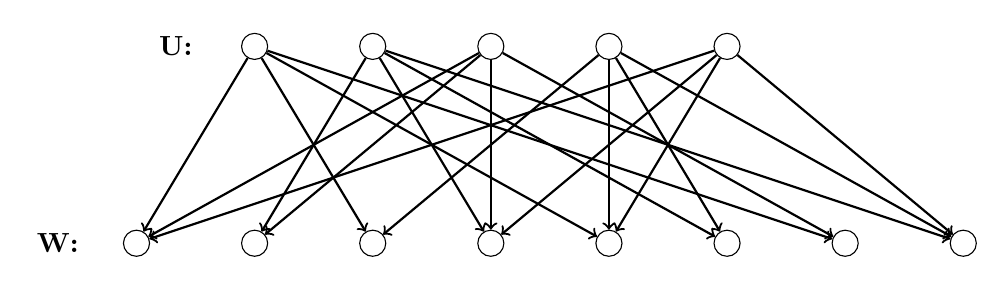
\begin{tikzpicture}
\tikzstyle{arrow}=[->, draw, thick]
\node[draw, circle] (v3) at (0,0) {};
\node[draw, circle] (v6) at (-4.5,-2.5) {};
\node[draw, circle] (v10) at (-3,-2.5) {};
\node[draw, circle] (v7) at (-1.5,-2.5) {};
\node[draw, circle] (v11) at (0,-2.5) {};
\node[draw, circle] (v8) at (1.5,-2.5) {};
\node[draw, circle] (v12) at (3,-2.5) {};
\node[draw, circle] (v9) at (4.5,-2.5) {};
\node[draw, circle] (v13) at (6,-2.5) {};
\node[draw, circle] (v2) at (-1.5,0) {};
\node[draw, circle] (v4) at (1.5,0) {};
\node[draw, circle] (v1) at (-3,0) {};
\node[draw, circle] (v5) at (3,0) {};
\node (v0) at (-4,0) {\textbf{U:}};
\node (v00) at (-5.5,-2.5) {\textbf{W:}};
    
\draw[arrow]  (v1) edge (v6);
\draw[arrow]  (v1) edge (v7);
\draw[arrow]  (v1) edge (v8);
\draw[arrow]  (v1) edge (v9);
\draw[arrow]  (v2) edge (v10);
\draw[arrow]  (v2) edge (v11);
\draw[arrow]  (v2) edge (v12);
\draw[arrow]  (v2) edge (v13);
\draw[arrow]  (v3) edge (v6);
\draw[arrow]  (v3) edge (v11);
\draw[arrow]  (v3) edge (v9);
\draw[arrow]  (v3) edge (v10);
\draw[arrow]  (v4) edge (v7);
\draw[arrow]  (v4) edge (v12);
\draw[arrow]  (v4) edge (v13);
\draw[arrow]  (v4) edge (v8);
\draw[arrow]  (v5) edge (v6);
\draw[arrow]  (v5) edge (v13);
\draw[arrow]  (v5) edge (v11);
\draw[arrow]  (v5) edge (v8);
\end{tikzpicture}
\end{figure}
$$\bbordermatrix{
&\Huge U &\Huge W\cr
\Huge U& \Huge O &\Huge H\cr
\Huge W & \Huge H^T & \Huge O 
}$$
Przypuśćmy, że graf $G$ jest ekspanderem.\\
Wtedy bardzo szybko można skorygować 2 błędy.
\begin{description}
\item[$U_1$] $|U|=100$, każdy wierzchołek $U$ jest połączony z 20 wierzchołkami z $W$
\item[$W_1$] $|W|=1000$
\end{description}
Taki graf (jeśli jest ekspanderem) potrafi skorygować nawet $5\%$ błędów.

\subsubsection{Liczenie średniej odległości}
\begin{theorem}[Metatwerdzenie]
Ekspander to rzadki graf który często ,,zachowuje się'' jak pełny.
\end{theorem}
\begin{proof}
Przypuśćmy, że mamy $n=10^5$ punktów, który jest ekspanderem.\\
Średnia odległość liczona po krawędziach tego grafu przybliża bardzo dobrze średnią odległość w liczonym grafie.
\end{proof}

\subsubsection{,,Zmniejszenie prawdopodobieństwa''}
\begin{theorem}[Małe twierdzenie Fermata]
$$a^{p-1}\equiv 1 (\mod p)$$
\end{theorem}
Przypuśćmy, że $n$ jest liczbą złożoną
$$a^{n-1}\equiv 1(\mod m)$$
dla co najwyżej potęgi liczb całkowitej produktu $[1;n-1]$
\begin{figure}[H]
\centering 
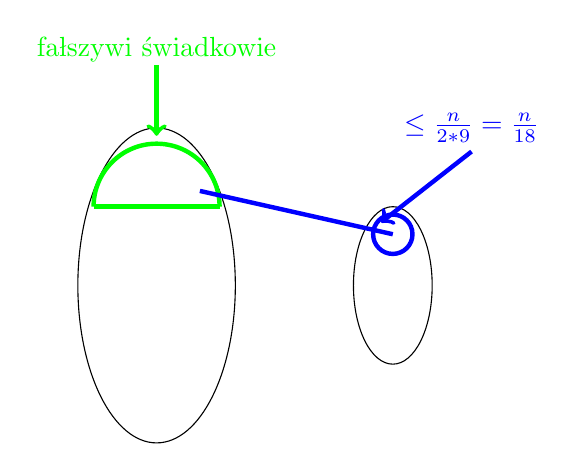
\begin{tikzpicture}
\draw  (0,0) ellipse (1 and 2);
\draw  (3,0) ellipse (.5 and 1);
\draw[ultra thick,color=green] (.8,1) arc (0:180:.8cm);
\draw[ultra thick,color=green] (-.8,1) -- (.8,1);
\node[color=green] at (0,3) {fałszywi świadkowie};
\draw[->,ultra thick,color=green] (0,2.8) -- (0,1.9);
\draw[ultra thick,color=blue]  (3,.65) ellipse (.25 and .25);
\draw[ultra thick,color=blue] (.55,1.2) -- (3,.65);
\node[ultra thick,color=blue] at (4,2) {$\leq \frac{n}{2*9}=\frac{n}{18}$};
\draw[->,ultra thick,color=blue] (4,1.7) -- (2.85,.8);
\end{tikzpicture}
\end{figure}
$d=10$ $|S|\leq \frac{n}{19}$ $|N(S)|> 9|S|$

I tak zamiast $\binom{1}{2}^k$ uzyskujemy $\binom{1}{19}^k$ 

%----------------------------------------------------------------
